\section{Introduction}
\begin{figure}[t]
\vspace{-0.7cm}
\centering

\includegraphics[width=0.35\textwidth]{picture/workflow.pdf}
\caption{Our GCL with spectral feature augmentation by the incomplete power iteration implicitly performs three steps. Let blue and red ellipses represent spectra of feature maps $\mathbf{H}^\alpha$ and $\mathbf{H}^\beta$  of two views. Singular values of unaligned views (top left) are firstly rebalanced (top right) and the noise is injected into singular values (bottom left). Given rebalanced singular values, corresponding singular vectors are aligned with equalized emphasis (leading unbalanced singular values would  emphasize the alignment of leading singular vectors, sacrificing the quality of alignment of other singular vectors).
\label{fig:implicit}
}
\vspace{-0.6cm}
\end{figure}
%The past few years have witnessed rapid advances in 
Semi-supervised and supervised Graph Neural Networks (GNNs) %, powerful learners for graphs
 \citep{velivckovic2017graph,hamilton2017inductive, song2022towards,zhang2022graph} require full access to class labels. However, unsupervised GNNs  \cite{klicpera2018predict,wu2019simplifying,zhu2021simple} and recent  Self-Supervised Learning (SSL) models do not  require  labels~\citep{song2021semi, DBLP:conf/ijcai/arvga} to train embeddings. Among SSL methods, Contrastive Learning (CL) achieves comparable performance with its supervised counterparts on many  tasks~\citep{chen2020simple,gao2021simcse}. CL has also been applied recently to the graph domain. A typical Graph Contrastive Learning (GCL) method forms multiple graph views via stochastic augmentation of the input to learn representations by contrasting so-called positive samples with negative samples~\citep{zhu2020deep,peng2020graph,zhu2021contrastive,zhu2021contrastive2,zhang2022costa}. As an indispensable part of GCL, the significance of graph augmentation has been well studied~\citep{hafidi2020graphcl,zhu2021graph,DBLP:journals/corr/autogcl}. 
% However, inappropriately designed graph augmentations might be ineffective due to undesired noise, or disrupted  data semantics/properties~\citep{DBLP:journals/corr/AdversaGA,DBLP:conf/nips/whatGoodVeiw}. Several authors~\citep{DBLP:journals/corr/autogcl, DBLP:conf/nips/whatGoodVeiw,DBLP:journals/corr/AdversaGA} proposed to learn graph augmentations which still require training with some supervision.
%
%However,  random data augmentations are problematic as their noise may be not relevant to downstream tasks~\citep{DBLP:journals/corr/AdversaGA,DBLP:conf/nips/whatGoodVeiw}. Some works ~\citep{DBLP:journals/corr/autogcl, DBLP:conf/nips/whatGoodVeiw,DBLP:journals/corr/AdversaGA} learn graph augmentations (supervision required).
%
Popular random data augmentations are just one strategy to construct views, and their noise may affect adversely downstream tasks~\citep{DBLP:journals/corr/AdversaGA,DBLP:conf/nips/whatGoodVeiw}. Thus, some works ~\citep{DBLP:journals/corr/autogcl, DBLP:conf/nips/whatGoodVeiw,DBLP:journals/corr/AdversaGA} learn graph augmentations but they require supervision.


The above issue motivates us to propose a simple/efficient data augmentation model %for GCL 
which is complementary with existing augmentation strategies. % and enhance the generalization ability. 
%One promising line of research 
We target Feature Augmentation (FA) as scarcely any FA works  exist in %to investigate FA in
the context of CL and GCL.
%
In the image domain, a simple FA~\citep{DBLP:conf/cvpr/UpchurchGPPSBW17,DBLP:conf/icml/BengioMDR13} showed that perturbing feature representations of an image results in a representation of another image where both images share some semantics~\citep{wang2019implicit}. 
%
However, perturbing features randomly ignores covariance of feature representations, and ignores semantics correlations. %and semantics remains mysterious in the graph domain due to the lack of visibility. 
Hence, we opt for injecting  random noise into the singular values of feature maps as such a spectral feature augmentation does not alter the orthogonal bases of feature maps by much, thus helping preserve semantics correlations. 

% For image, simple feature augmentation can be achieve via add small random noise to the hidden feature maps. This move original image toward a random direction in the hidden space, resulting in another image with similar semantics. But such property remains mysterious to graph domain as the lack of visibility. We opt for injecting 
% random noise to the spectrum of feature map as it does not alter the subspace keeping the semantics relatively uncharged after augmentation. 

%  In this paper, we propose a novel FA approach for GCL via perturbing the spectrum of the graph view. 
%  We notice that the barrier to improving the model generalization ability and accuracy is due to the large singular value gap and the unbalanced spectrum of the graph views. 
%  Typical GCL requires aligning of the two correlated views~\citep{wang2020understanding}. However, it may become difficult to optimize the alignment of two correlated views with unbalanced singular value since the largest singular value may dominate the alignment process. As a result, the model will focus on aligning the singular vector corresponding to the largest singular value and negligible alignment is imposed on other orthogonal directions with small singular values. In other words, the unbalanced spectrum causes a suboptimal orthonormal bases alignment giving rise to a suboptimal solution of the GCL model. To this end, we design a FA to reduce the singular value gap and balance the spectrum via assigning a smaller/larger scale factor to a larger/smaller singular value of the feature map. We evaluate our method on various datasets for node classification. Our results indicate that using graph augmentation with our proposed approach significantly improves  the accuracy and generalization ability in comparison to counterpart baseline models. 

% \begin{figure*}[t]
% \vskip 0.2in
% \centering
% \begin{subfigure}[b]{0.82\textwidth}
% \centerline{
\includegraphics[width=\textwidth]{picture/framework.pdf}}
% \caption{\label{fig:frama}}
% \end{subfigure}
% \hspace{0.1cm}
% \begin{subfigure}[b]{0.156\textwidth}
% \centerline{\includegraphics[width=\textwidth]{picture/steps.pdf}}
% \caption{\label{fig:framb}}
% \end{subfigure}
% \caption{A proposed GCL model is in Fig \ref{fig:frama}. Two graph views are generated via data augmentation functions. Subsequently, two graphs are passed into graph neural network encoders with shared parameters to learn node representations. The proposed spectral feature augmentation balances (partially equalizes) the spectrum of each feature map, and implicitly injects the noise into the singular values. Such representations are fed into the projection head and the contrastive loss. Fig. \ref{fig:framb} illustrates the feature alignment process.}
% \label{fig:framework1}
% \vskip -0.2in
% \end{figure*}
 \begin{figure*}
 \centering
 \begin{subfigure}[b]{0.65\textwidth}
   % 
\includegraphics[width=0.9\textwidth,
   % height=2.9cm]{picture/framework.pdf}
   
\includegraphics[width=0.9\textwidth]{picture/framework.pdf}
    \caption{Our pipeline.\label{fig:framework1}}
    \end{subfigure}
    \begin{subfigure}[b]{0.25\textwidth}
    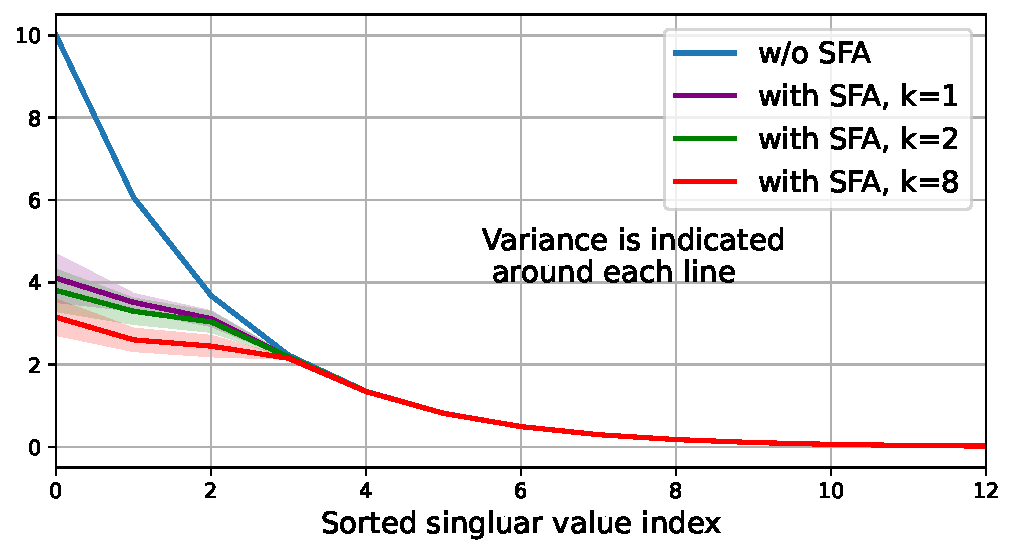
\includegraphics[width=\textwidth,height=3cm]{picture/fig.pdf}
    \caption{Simulation: spectrum obtained by Alg.~\ref{algo:1}.$\!\!\!$\label{fig:simulation}}
    \end{subfigure}
\vspace{-0.2cm}
\caption{Our GCL model. Two graph views are generated by data augmentation and passed into graph neural network encoders with shared parameters to learn node representations. The proposed spectral feature augmentation rebalances (partially equalizes) the spectrum of each feature map, and implicitly injects the noise into rebalanced singular values. Such representations are fed into the projection head and the contrastive loss. Figure~\ref{fig:implicit} explains the role of our spectral feature augmentation.}
%\vskip -0.2in
\end{figure*}


Moreover, as typical GCL aligns two data views~\citep{wang2020understanding}, unbalanced singular values of two data views may affect the quality of alignment. As several leading singular values  (acting as weights on the loss) dominate the alignment process, GCL favors aligning the leading singular vectors of two data views while sacrificing remaining orthogonal directions with small singular values. In other words, the unbalanced spectrum leads to a suboptimal orthonormal bases alignment, which results in a suboptimal GCL model.

To address rebalancing of unbalanced spectrum and augmenting leading singular values, we present a novel and efficient {\em Spectral Feature Augmentation} (SFA).
%\textbf{S}pectral \textbf{F}eature \textbf{A}ugmentation (SFA).
To this end, we propose the so-called incomplete power iteration which, under just one or two iterations, partially balances singular values of feature maps and implicitly injects the noise into these singular values. %For two views, we align these complement feature maps as the spectrum-balanced alignment step focuses on less dominant singular values of spectra of both views, whereas the spectral augmentation of values does not affect the spectral angle alignment (singular vectors are left intact). We evaluate our method on various datasets for node level tasks (\ie, node classification and node clustering). Our results indicate that using graph augmentation with our proposed approach significantly improves the accuracy and generalization ability in comparison to counterpart baseline models. 
We evaluate our method on various datasets for node level tasks (\ie, node classification and node clustering). We also
show that our  method is compatible with other augmentation strategies and contrastive losses.

\vspace{0.15cm}

We summarize our contributions as follows:
%\vspace{-0.15cm}

\renewcommand{\labelenumi}{\roman{enumi}.}
%\vspace{-1.0mm}
%\hspace{-1.5cm}
\begin{enumerate}[leftmargin=0.5cm]
     \item We propose a simple/efficient spectral feature augmentation for GCL which is independent of different contrastive losses, \ie, we employ %of contrastive loss (\ie, InfoNCE) and non-contrastive loss (Barlow Twin) 
     InfoNCE and Barlow Twin.
     %in the graph domain.
     %The spectral augmentation is perfromed 
     \vspace{-0.1cm}
     \item We introduce the so-called incomplete power iteration which, under just one or two iterations, partially  balances  spectra of two data views and injects the augmentation noise into their singular values. The rebalanced spectra help align orthonormal bases  of both data views.
    %  and analyze the relation between the structural noise added in the feature matrix spectrum and the noise in feature matrix.
     \vspace{-0.1cm}
     \item As the  incomplete power iteration is stochastic in its nature, %we show it can balance the spectrum and inject the noise into singular values, 
     we derive its analytical form which provably demonstrates its spectrum rebalancing effect in expectation, and captures the variance of the spectral augmentation.
     \vspace{-0.1cm}
     \item For completeness, we devise other spectral augmentation models, based on the so-called MaxExp and Power Norm. operators and Grassman feature maps, whose rebalancing and noise injection profiles differ with our method. 
     %\item We show experimentally that our method prevents the dimensional collapse and demonstrates competitive performance on different datasets. Notably, our  method is also compatible with data augmentation strategies.
 \end{enumerate}
 
 
% \subsubsection{Augmentations}
 


% Recent works in self-supervised graph learning suggest that contrasting congruent and incongruent views of graph allows encoders to learn rich representations. Different graph view are generated by add random permutation to the sturtcure and attribute of the graph (i.e.,,, edge droping , attribute masking). However, graph augmentation is sensitive to the setting of the random perturbation (i.e.,, the dropping/masking ratio) and may incorporate unrelated noise to the pretrain features~\ref{}. Hence, we opted for doing extra augmentation on the hidden features.

% We empirically show that in most cases the best results are
% achieved by further adding random noise to thee spetrun of the features maps obtain from graph augmentation and treating the result augmented features maps as two congruent views of same graph’s structure (see section 4.4). We speculate that because adjacency and diffusion matrices provide
% local and global views of a graph structure, respectively,
% maximizing agreement between representation learned from
% these two views allows the model to simultaneously encode
% rich local and global information.